\subsection{High-level components and their interaction}

The main software components forming the system, the interfaces provided and required from the software units, along with the relationship of necessity between components, are shown in the component diagram below [figure \ref{fig:high-lev-comp-diag}].

Note that not all the components represented, like the browser, are actually software units of the final system, but are part of the environment with which the system will interact.

\begin{figure}[h]
	\centerline{
		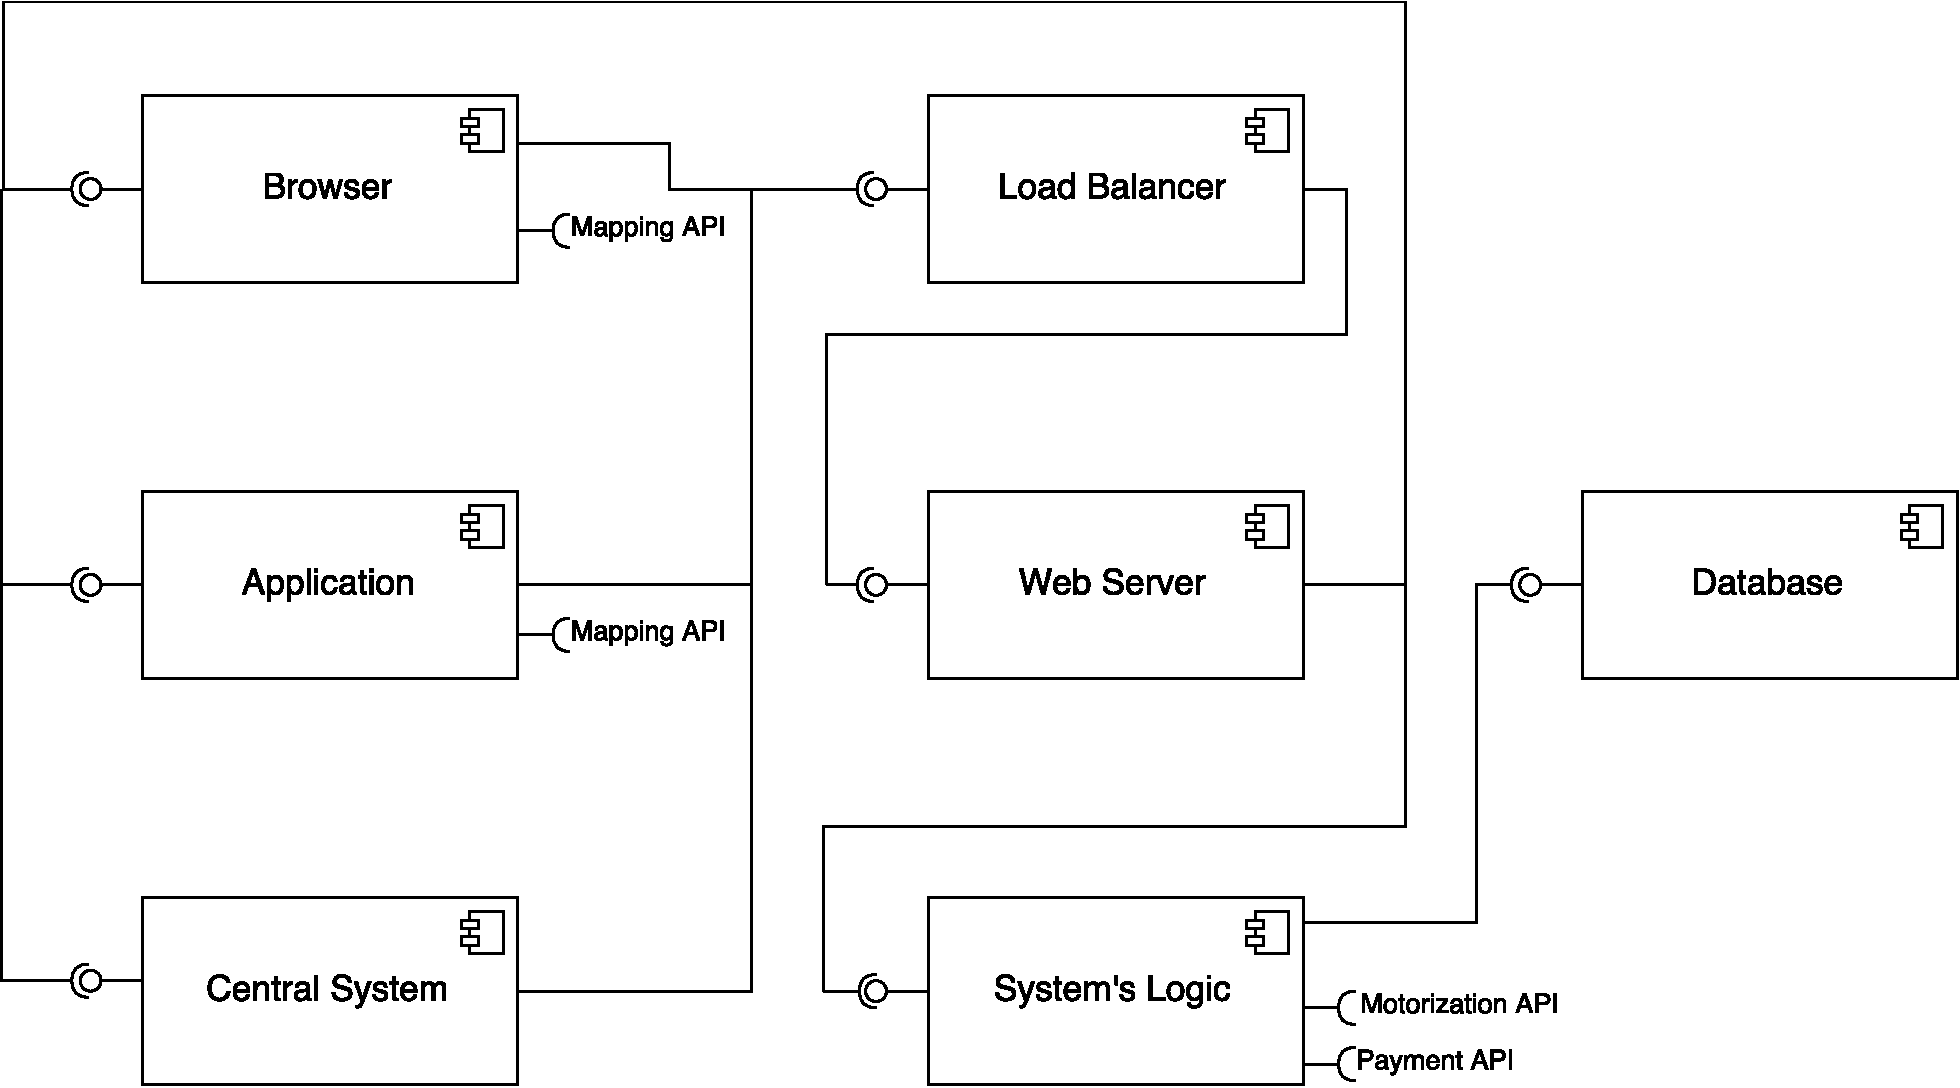
\includegraphics[width=400px]{../Datas/images/high-level-component-diagram.pdf}
	}
	\caption{High-level component diagram}
	\label{fig:high-lev-comp-diag}
\end{figure}

\begin{itemize}
	\item \textbf{Browser}: The software used by the user to access to the service.
	\item \textbf{Mobile application}: the application installed on mobile devices and used by the user to access to the service.
	\item \textbf{Central system}: also called Car's Central System. It's the software responsible for car's management and interfacing with the system.
	\item \textbf{Load balancer}: the software used to distribute the workload to the servers.
	\item \textbf{Web server}: the software used to elaborate requests and send back responses.
	\item \textbf{System's logic}: the software responsible for the whole system's logic.
	\item \textbf{Database}: the software unit responsible for the management of queries and data.
\end{itemize}
